\section{Lecture 1}

\subsection{Robotics History}

\begin{definition}[Robot, Robotics]
    A robot is a "mechanical device" that sometimes resembles a human and is capable of performing a variety of often complex human taks.

    Robotics is the science and building of robots.
\end{definition}

The CAMSF function block model:

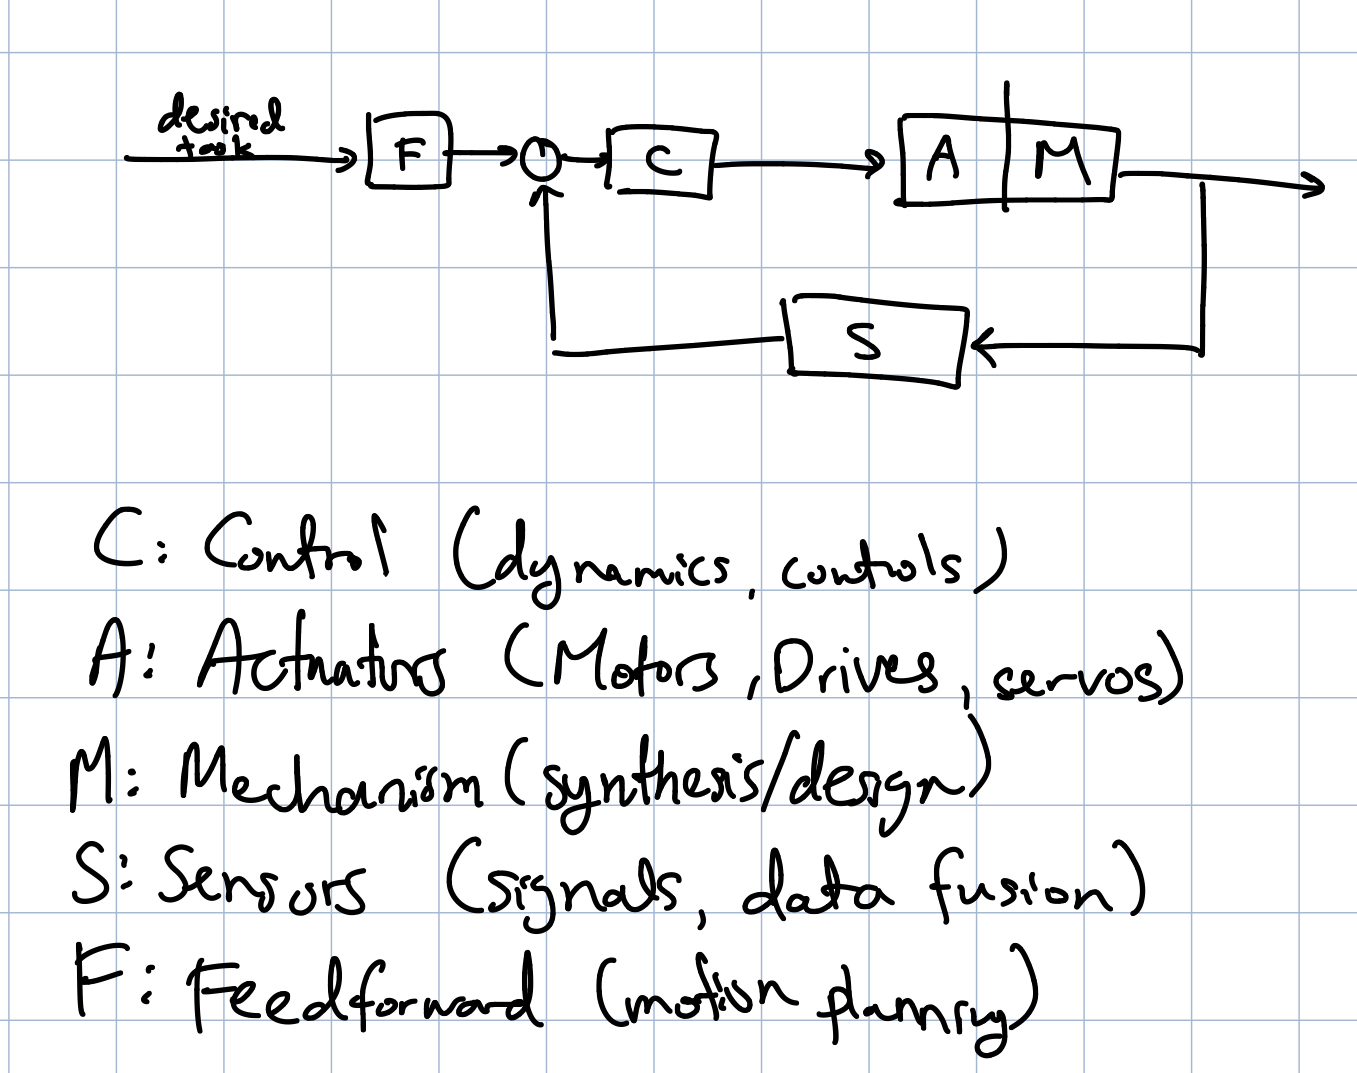
\includegraphics[width=250px]{../images/blockorigin.jpeg}

In ancient history (the Egyptians, Greeks, Romans), simple machines such as inclined planes, levers, pullies, capstands and cranks. These mechanisms
relied on multiplying force using some kind of mechanical ratios (whether by trading off distance, energy, etc).